Praca opiera się na wykorzystaniu języka R oraz Python do generowania zbiorów danych, wszelkich manipulacji na nich oraz ich klasyfikacji.

\begin{figure}[ht]
	\centering
	
\includegraphics[height=2cm]{partials/images/logo_r.png}
	\caption{Logo R}
\label{Fig:R}
\end{figure}

Język R~to szeroko stosowany w~statystyce, analizie danych oraz naukach przyrodniczych język interpretowalny.
Nie ma on skomplikowanej składni i jest przystosowany do bycia jak najbardziej przyjaznym dla nowego użytkownika.
Oprócz dużych możliwości obliczeniowych, jest również świetnym narzędziem do wizualizacji danych,
co spowodowało, że został wybrany do stworzenia zbioru danych.
Grafy wygenerowane zostały przy pomocy biblioteki igraph w wersji~2.0.3.
Jest to pakiet do tworzenia i~analizy struktur sieci, a co za tym idzie oferuje bogaty wybór funkcji do
generowania losowych i~regularnych grafów oraz ich wizualizacji.

\begin{figure}[ht]
	\centering
	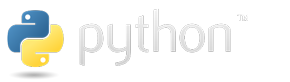
\includegraphics[height=2cm]{partials/images/logo_python.png}
	\caption{Logo Python}
\label{Fig:Python}
\end{figure}

Język Python jest jednym z najpopularniejszych języków wysokopoziomowych ogólnego przeznaczenia.
Zawdzięcza to swojej wszechstronności oraz prostocie składni.
Znaczna liczba bibliotek pozwala na wykorzystywanie Pythona od
prostych skryptów, przez analizę danych, aż po rozbudowane aplikacje, takie jak całe
systemy największych gigantów technologicznych, np. Google. Język ten jest szeroko
wykorzystywany w dziedzinie Data Science do wizualizacji, analizy~i przetwarzania danych oraz w uczeniu maszynowym.
Ostatnie z wymienionych zastosowań zadecydowało~o wyborze języka Python jako narzędzia do stworzenia modelu klasyfikacji grafów.
Wykorzystana została biblioteka Keras z pakietu Tensorflow.